\section{Proposed Architecture}
\label{sec:solution_architecture}

This chapter presents the architecture of the proposed intelligent medical image analysis framework. The system is designed as a hierarchical, modality-aware diagnostic pipeline capable of analyzing heterogeneous medical imaging data while maintaining high levels of reliability, interpretability, and scalability. The architecture addresses a practical challenge frequently encountered in real-world clinical environments: different diseases are diagnosed using different imaging modalities, and therefore a single monolithic model may not be the most effective solution. Instead, the proposed framework decomposes the overall diagnostic task into a sequence of specialized stages that collectively form an end-to-end decision-making pipeline.

The framework has been designed to support the automated analysis of chest radiographs and computed tomography (CT) scans. More specifically, the system is capable of detecting COVID-19, Tuberculosis, and Pneumonia from chest X-ray images, while also performing lung cancer detection from CT scans. In addition to disease classification, the framework incorporates Explainable Artificial Intelligence (XAI) mechanisms to improve transparency and trustworthiness, as well as Federated Learning (FL) capabilities to facilitate privacy-preserving collaborative model development across multiple healthcare institutions.

The overall architecture follows a two-level classification paradigm. At the first level, an intelligent routing model determines the modality of the incoming image and verifies whether it belongs to one of the supported image categories. At the second level, modality-specific diagnostic models perform disease prediction. This hierarchical structure enables the system to leverage specialized classifiers that are optimized for their respective tasks while reducing the complexity associated with training a single generalized model.

Figure~\ref{fig:full_overall_architecture} presents a high-level overview of the proposed framework.

\begin{figure}[H]
	\centering
	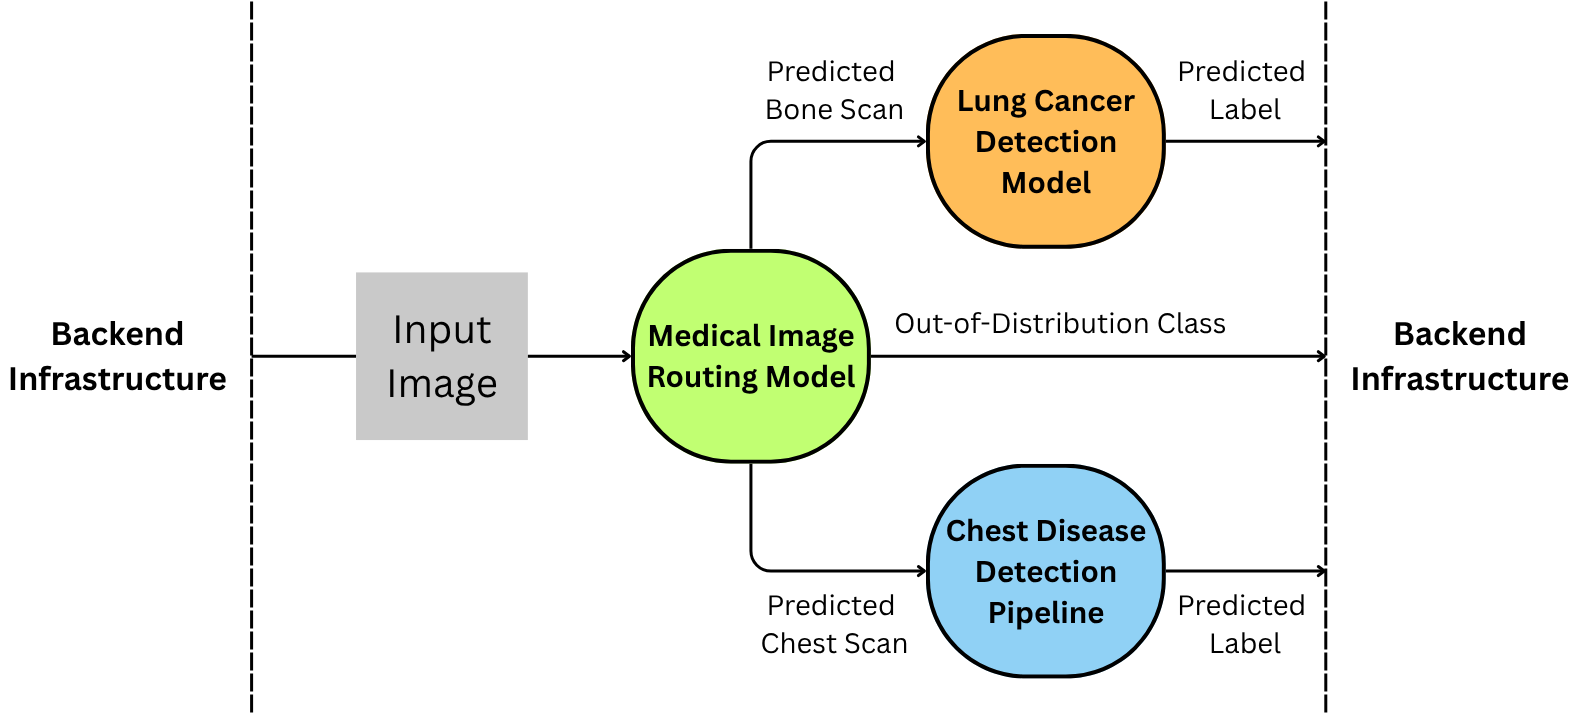
\includegraphics[width=\linewidth]{assets/full_project_arch.png}
	\caption{High-level architecture of the proposed framework. The system consists of a modality routing model, specialized disease classifiers, Explainable AI modules, and a Federated Learning infrastructure connecting multiple healthcare institutions.}
	\label{fig:full_overall_architecture}
\end{figure}

\subsection{Architectural Design Philosophy}

The proposed framework was developed according to several architectural principles that were established at the beginning of the system design process. These principles were intended to ensure that the resulting framework would not only achieve strong predictive performance but would also remain practical for real-world deployment in healthcare environments.

One of the most important design considerations was modality awareness. Medical images generated by different imaging technologies exhibit fundamentally different visual characteristics and diagnostic properties. Chest radiographs provide projection-based representations of thoracic structures, whereas CT scans generate detailed cross-sectional views that reveal significantly more anatomical information. These differences influence the types of features that neural networks must learn in order to perform accurate diagnosis. A single generalized model trained across multiple modalities may struggle to simultaneously learn optimal representations for all imaging types. Consequently, the proposed architecture explicitly separates modality identification from disease diagnosis. This design allows each diagnostic model to focus exclusively on data originating from the modality for which it was designed.

Another fundamental design principle was task specialization. The diseases targeted by this work differ substantially in terms of pathological manifestations, imaging characteristics, and diagnostic requirements. COVID-19, Tuberculosis, and Pneumonia are primarily identified using chest radiographs, whereas lung cancer diagnosis often relies on the higher anatomical resolution available in CT imaging. Rather than attempting to train a single network to recognize all diseases across all modalities, the proposed framework distributes these tasks among specialized models. This decomposition reduces task complexity and allows each model to learn more discriminative feature representations relevant to its specific diagnostic objective.

Reliability and patient safety also played a significant role in the architectural design. Medical AI systems must operate in environments where unexpected inputs are inevitable. Hospital information systems frequently contain diverse imaging studies, and a deployed diagnostic model may encounter unsupported image types, corrupted files, incomplete scans, or non-medical images. If such inputs are processed without validation, the resulting predictions may be unreliable and potentially dangerous. To address this issue, the proposed framework incorporates an explicit out-of-distribution detection mechanism within the routing stage. This component enables the system to identify unsupported inputs before they reach the diagnostic models.

Transparency represents another critical requirement for healthcare AI systems. Clinical practitioners often require evidence supporting automated predictions before integrating them into their decision-making processes. While deep neural networks have demonstrated remarkable predictive capabilities, they are frequently criticized for their lack of interpretability. The proposed architecture therefore integrates explainability mechanisms directly into the diagnostic workflow. These mechanisms provide visual explanations that highlight image regions contributing to the final prediction, thereby allowing clinicians to better understand and validate the reasoning process of the model.

Finally, the architecture was designed with scalability and long-term deployment in mind. Healthcare institutions are often unable to share patient data due to privacy regulations, legal restrictions, and ethical concerns. Consequently, the framework incorporates Federated Learning capabilities that enable multiple institutions to collaboratively improve model performance without exchanging raw patient information. This design promotes the creation of a continuously improving diagnostic ecosystem while preserving patient confidentiality.

\subsection{System Workflow}

The complete workflow of the proposed framework begins when a medical image is submitted to the system. Following acquisition, the image undergoes preprocessing operations intended to standardize the input format and improve compatibility with the downstream neural networks. These operations may include resizing, normalization, intensity standardization, and other transformations required by the underlying deep learning models.

Once preprocessing is completed, the image is forwarded to the first level of the architecture, namely the modality routing model. The purpose of this stage is to determine the nature of the input image and identify the appropriate diagnostic pathway. The routing decision governs all subsequent processing stages and therefore serves as a critical component of the framework.

After the routing decision is generated, the image is directed toward a specialized diagnostic model. Images identified as chest radiographs are analyzed by the chest disease classifier, while CT scans are analyzed by the lung cancer detection model. Images identified as out-of-distribution are excluded from automated diagnosis and may instead be flagged for manual review by healthcare personnel.

Following disease prediction, explainability modules generate visual interpretations of the model output. These interpretations provide insight into the image regions that most strongly influenced the prediction process. Finally, the prediction and associated explanation are presented to the clinician. During model training, Federated Learning mechanisms facilitate collaborative model improvement across multiple participating institutions.

Figure~\ref{fig:classification_tree} illustrates the classification pathway implemented by the proposed framework.

\begin{figure}[H]
	\centering
	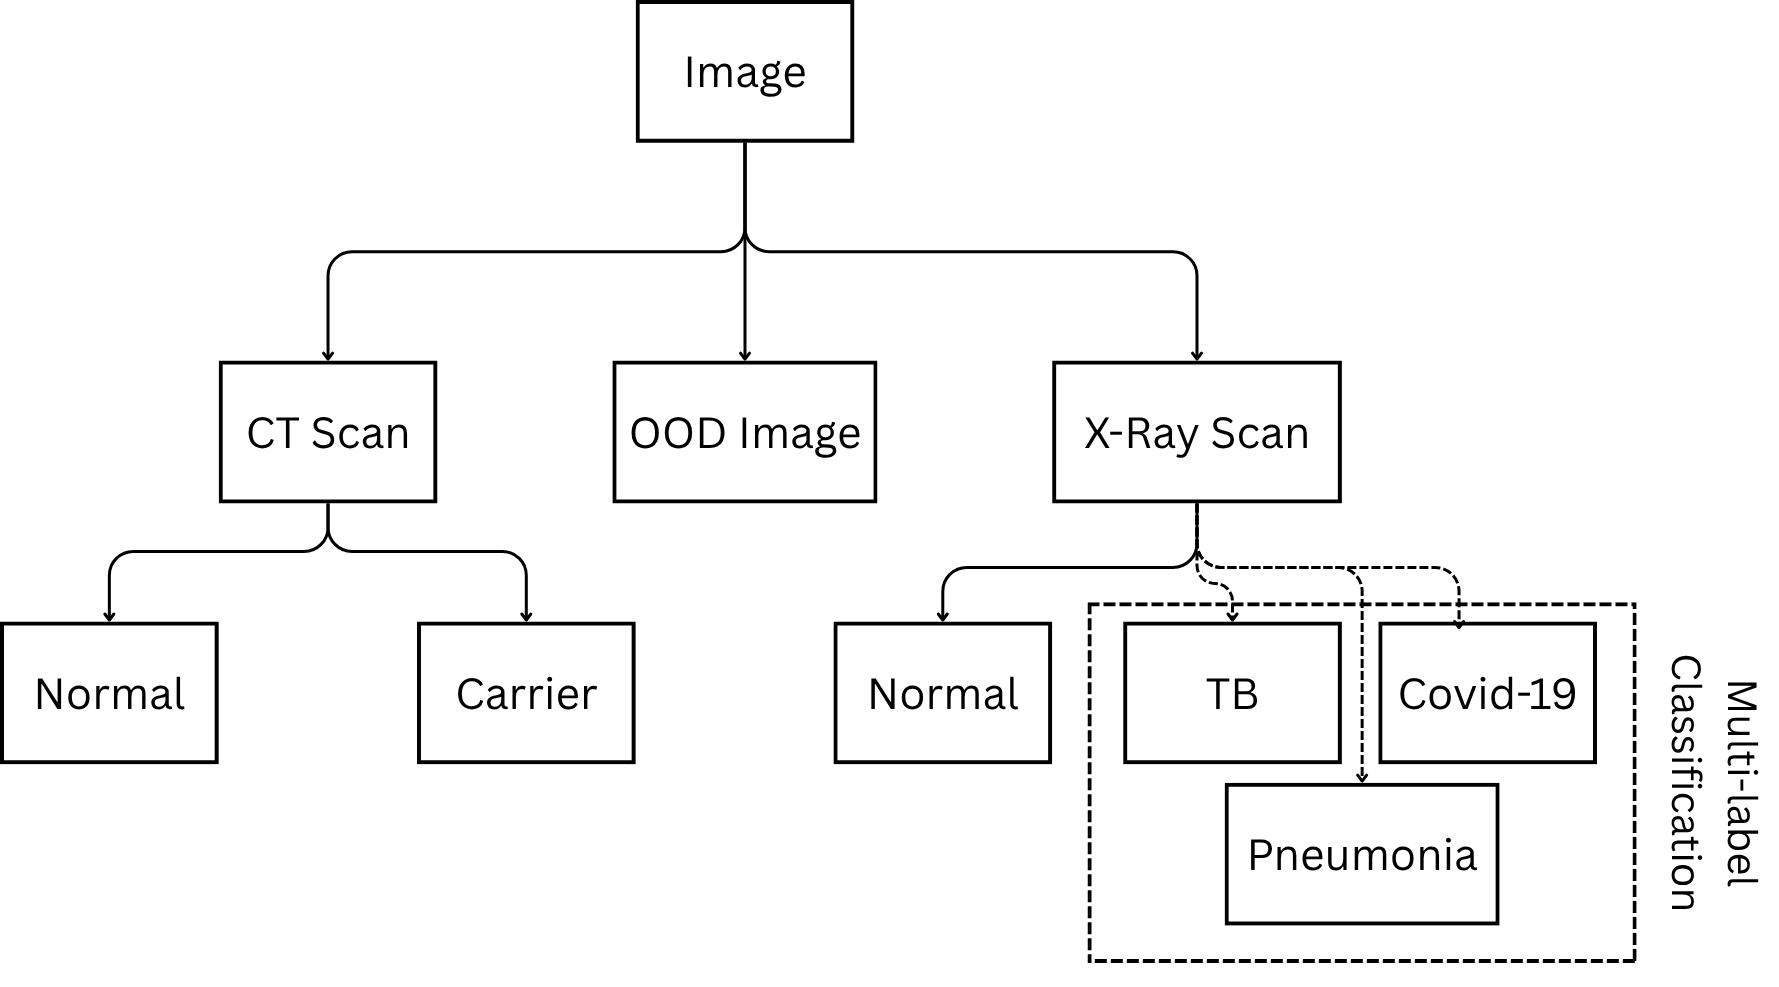
\includegraphics[width=0.8\linewidth]{assets/classification_tree.png}
	\caption{Classification tree of the proposed two-level framework. The routing model first determines the image modality before directing the image toward the appropriate disease-specific classifier.}
	\label{fig:classification_tree}
\end{figure}

\subsection{Level One: Modality Routing and Out-of-Distribution Detection}

The first level of the proposed architecture functions as an intelligent routing mechanism responsible for identifying the modality of the incoming image. Although this component performs a relatively simple classification task compared to disease diagnosis, its importance should not be underestimated. Every subsequent prediction generated by the framework depends directly on the correctness of the routing decision.

Formally, let $I$ denote an input image. The routing model $R(\cdot)$ maps the image into one of three categories:

\begin{equation}
	R(I) \in \{\text{X-ray}, \text{CT}, \text{OOD}\}
\end{equation}

where OOD represents an out-of-distribution image.

The motivation for introducing a dedicated routing stage arises from the substantial differences between X-ray and CT imaging modalities. Chest radiographs represent two-dimensional projection images that summarize anatomical information along a viewing direction. In contrast, CT scans provide detailed cross-sectional information that enables the visualization of internal structures with considerably greater precision. These differences imply that the features required for effective diagnosis are modality-dependent. Routing images to specialized models therefore allows the framework to exploit modality-specific representations rather than relying on a generalized feature extraction strategy.

From a computational perspective, routing also improves efficiency. Without this stage, every image would need to be processed by every available diagnostic model, resulting in increased computational cost and unnecessary inference overhead. By ensuring that each image is evaluated only by the most relevant classifier, the routing model reduces resource consumption and improves scalability.

An equally important function of the routing stage is out-of-distribution detection. In practical deployment scenarios, healthcare systems may receive images that differ significantly from those used during training. Examples include magnetic resonance imaging studies, ultrasound images, pathology slides, non-medical photographs, or improperly formatted files. Diagnostic models are generally incapable of producing reliable predictions for such inputs because they fall outside the distribution of the training data.

To mitigate this problem, the routing model incorporates a dedicated OOD category. Images assigned to this category are prevented from entering the diagnostic pipeline. This safeguard reduces the likelihood of erroneous predictions and contributes to the overall reliability of the framework. From a clinical perspective, this mechanism functions as a preliminary quality-control layer that ensures only supported image types proceed to automated analysis.

\subsection{Level Two: Chest Disease Detection Model}

Images identified as chest radiographs are forwarded to the chest disease classification model. This model is responsible for detecting three clinically significant respiratory diseases: COVID-19, Tuberculosis, and Pneumonia.

The selection of these diseases was motivated by both clinical relevance and public health importance. COVID-19 remains one of the most extensively studied respiratory illnesses in recent years and has highlighted the importance of rapid imaging-based screening techniques. Tuberculosis continues to represent a major global health challenge, particularly in developing countries where early detection plays a crucial role in disease management and transmission control. Pneumonia remains one of the most common respiratory infections worldwide and is associated with substantial morbidity and mortality across multiple age groups.

A key characteristic of the proposed chest disease model is its formulation as a multi-label classification problem rather than a conventional multi-class classification problem. This distinction is essential because the targeted diseases are not mutually exclusive. In clinical practice, a patient may simultaneously exhibit radiological findings associated with multiple respiratory conditions. For example, viral infections may be accompanied by secondary bacterial pneumonia, and complex pathological interactions may lead to overlapping imaging manifestations.

Traditional multi-class classification assumes that each sample belongs to exactly one category. Such an assumption would force the model to select a single disease label even when multiple diseases are present. This formulation would therefore fail to accurately represent many real-world clinical scenarios.

To address this limitation, the proposed architecture employs independent disease predictions. Let

\begin{equation}
	\mathbf{y} =
	[y_{\text{COVID}}, y_{\text{TB}}, y_{\text{Pneumonia}}]
\end{equation}

denote the output vector generated by the classifier. Each element corresponds to the estimated probability that a specific disease is present within the image.

Unlike a softmax-based multi-class architecture, the output layer uses independent sigmoid activations. This allows the model to assign high probabilities to multiple diseases simultaneously whenever appropriate. The final prediction for each disease is obtained by applying a predefined threshold:

\begin{equation}
	\hat{y}_i=
	\begin{cases}
		1 & y_i \geq \tau \\
		0 & y_i < \tau
	\end{cases}
\end{equation}

where $\tau$ denotes the classification threshold.

This formulation better reflects the realities of clinical diagnosis and provides greater flexibility when interpreting model outputs. Instead of receiving a single categorical prediction, clinicians are presented with independent disease probabilities that can be incorporated into broader diagnostic assessments.

\subsection{Level Two: Lung Cancer Detection Model}

Images classified as CT scans are forwarded to the lung cancer detection model. The decision to utilize CT imaging for lung cancer analysis is motivated by the superior anatomical detail provided by computed tomography compared to conventional radiography.

Lung cancer frequently manifests through subtle structural abnormalities such as pulmonary nodules, irregular masses, and localized tissue changes that may not be visible in chest radiographs. The high spatial resolution of CT imaging enables these features to be observed with significantly greater clarity, making CT the preferred modality for many lung cancer screening and diagnostic procedures.

The objective of the lung cancer model is to determine whether cancer-related findings are present within the input scan. The classifier can be represented mathematically as

\begin{equation}
	P_{\text{Cancer}} = C(I)
\end{equation}

where $C(\cdot)$ denotes the lung cancer detection network and $P_{\text{Cancer}}$ represents the estimated probability of malignancy.

By focusing exclusively on CT-derived information, the model can dedicate its representational capacity to learning highly discriminative cancer-related features. This specialization improves the model's ability to identify subtle pathological patterns that may be difficult to detect using a generalized classifier.

\subsection{Explainable Artificial Intelligence Integration}

The increasing adoption of artificial intelligence within healthcare has generated significant interest in model interpretability. Although deep learning systems are capable of achieving remarkable predictive performance, their internal decision-making processes often remain difficult to understand. This lack of transparency can hinder clinical adoption, particularly when predictions influence critical healthcare decisions.

To address this challenge, Explainable Artificial Intelligence techniques are integrated directly into the proposed architecture. Rather than treating explainability as an optional post-processing step, it is considered a fundamental component of the diagnostic workflow.

Following prediction generation, the explainability module produces visual explanations illustrating the regions of the image that most strongly influenced the model's decision. These visualizations may take the form of saliency maps, activation maps, attention maps, or gradient-based explanations depending on the selected implementation.

The integration of explainability serves several purposes. First, it increases clinician confidence by providing visual evidence supporting the model's prediction. Second, it facilitates model validation by enabling researchers to verify that the network is focusing on medically meaningful regions rather than irrelevant artifacts. Third, it assists in identifying potential biases or failure modes that may otherwise remain hidden within the network. Ultimately, explainability strengthens the collaborative relationship between clinicians and AI systems by transforming predictions into interpretable decision-support information.

\subsection{Federated Learning Infrastructure}

A distinguishing feature of the proposed framework is its support for Federated Learning. This capability was incorporated to address one of the most significant challenges facing medical artificial intelligence: limited access to large and diverse datasets.

Traditional deep learning systems typically rely on centralized training approaches in which data from multiple institutions are collected and stored in a single repository. While effective from a machine learning perspective, this strategy introduces substantial privacy, security, and regulatory concerns. Healthcare organizations are often prohibited from sharing patient data due to legal and ethical restrictions.

Federated Learning offers an alternative paradigm in which training occurs locally at each institution. Rather than transmitting patient data, participating hospitals train local models using their own datasets and share only model parameters or parameter updates. These updates are subsequently aggregated to produce a global model.

Let $w_i$ denote the model parameters learned by institution $i$, and let $n_i$ denote the number of training samples available at that institution. Using the Federated Averaging algorithm, the global model is computed as

\begin{equation}
	w_{\text{global}}
	=
	\sum_{i=1}^{K}
	\frac{n_i}{\sum_{j=1}^{K}n_j}
	w_i
\end{equation}

where $K$ represents the total number of participating institutions.

Beyond privacy preservation, Federated Learning provides several additional benefits. Because participating institutions often serve different patient populations, the resulting datasets contain greater demographic, geographic, and clinical diversity. Training across such heterogeneous data sources can improve model generalization and reduce susceptibility to institution-specific biases. Furthermore, the collaborative nature of Federated Learning enables continuous improvement of the framework as new institutions join the network and contribute additional knowledge.
